%% ****** Start of file rsitemplate.tex ****** %
%%
%%   This file has been edited from the original source file.
%%	 The original file is part of the revtex4-1 package indicated below.
%%   Version 4.1 of 9 October 2009.
%%
%
% This is a template for producing documents for use with 
% the REVTEX 4.1 document class and the RSI substyle.
% 
% Copy this file to another name and then work on that file.
% That way, you always have this original template file to use.

%\documentclass[aip,rsi,preprint,graphicx]{revtex4-1} % for checking your page length
\documentclass[aip,rsi,preprint,graphicx]{revtex4-1} % for review purposes
\usepackage{hyperref}
\usepackage{graphicx}

\draft % marks overfull lines with a black rule on the right

\begin{document}

% Use the \preprint command to place your local institutional report number 
% on the title page in preprint mode.
% Multiple \preprint commands are allowed.
%\preprint{}

\title{Short-cycle fast temperature program gas chromatograph for SFC$\times$GC} %Title of paper

% repeat the \author .. \affiliation  etc. as needed
% \email, \thanks, \homepage, \altaffiliation all apply to the current author.
% Explanatory text should go in the []'s, 
% actual e-mail address or url should go in the {}'s for \email and \homepage.
% Please use the appropriate macro for the type of information

% \affiliation command applies to all authors since the last \affiliation command. 
% The \affiliation command should follow the other information.

\author{D Malan}
\email[]{niel.malan@scidat.co.za}
\homepage[]{www.scidat.co.za}
%\thanks{}
%\altaffiliation{}
\affiliation{Department of Chemistry, University of Pretoria}

\author{ER Rohwer}
\email[]{egmont.rohwer@up.ac.za}
%\homepage[]{Your web page}
%\thanks{}
%\altaffiliation{}
\affiliation{Department of Chemistry, University of Pretoria}


% Collaboration name, if desired (requires use of superscriptaddress option in \documentclass). 
% \noaffiliation is required (may also be used with the \author command).
%\collaboration{}
%\noaffiliation

\date{\today}

\begin{abstract}
We present a fast chromatographic system that can be used as a second dimension in comprehensively coupled supercritical fluid chromatography/gas chromatography. The short (1 metre long) capillary column is heated by a resistively heated coaxial stainless steel tube. The temperature of the stainless steel is measured by determining the resistance through the current/voltage ratio. Heating rates of up to 2100 C$^\circ$/min (35 C$^\circ$/s) are obtained. To reduce the cooling time between temperature programs the coaxial heater is cooled by injecting evaporating carbon dioxide into the space between the coaxial heater and the column. This gives cooling rates of 5100 C$^\circ$/min (85 C$^\circ$/s) which allows very rapid repetition of temperature programmes.
\end{abstract}

\pacs{}% insert suggested PACS numbers in braces on next line
{82.80.Bg}

\maketitle %\maketitle must follow title, authors, abstract and \pacs

% Body of paper goes here. Use proper sectioning commands. 
% References should be done using the \cite and \label commands

\section{Introduction}
\label{Introduction}
% Niel: Literature review

\subsection{Heating for chromatography}

Comprehensive two-dimensional chromatography has become a well-established technique in analytical chemistry, in the form of GC$\times$GC and LC$\times$LC. Some other comprehensive techniques that are still looking to progress beyond the laboratory are LC$\times$SFC and SFC$\times$GC. These systems depend on orthogonality: the second dimension separation must use a significantly different separation mechanism than the first dimension.

When a gas chromatographic second dimension separation is used that is totally orthogonal to the first dimension, then the second dimension will run into the general elution problem: it becomes unlikely that one set of acceptable operating conditions (temperature, flow and stationary phase) will give acceptable (fast enough and with adequate resolution) separation.

In GC$\times$GC as it is practiced today, this has become a real problem. Wraparound is a well-known phenomenon in GC$\times$GC\cite{Dalluege2003}. This happen when a peak or peaks elute `late' on the second dimension, so late that the next modulation period has already started before it elutes, so that the peak comes out on the next D$^2$ chromatogram. This is, ironically, the result of high orthogonality. There are ways to avoid or ignore wraparound, but using a temperature program in the second dimension would make it in principle possible to remove all wraparound. 

If wraparound is a problem in GC$\times$GC, it becomes inevitable in SFC$\times$GC. The first dimension (SFC) does not necessarily separate compounds in a way that correlates with boiling point. Indeed, SFC is particularly good in making group-type separations\cite{Venter1999}, where compounds with a wide range of boiling points but with similar polarity elute together. 

Temperature programming is the usual way of getting around the general elution problem. However, in practical 2D chromatography the second dimension must be fast, which requires a short column and a high carrier flow. Since the recommended heating rate is around 10 C$^\circ$ per void time\cite{Blumberg2000}, the short column and high elution rate makes void times short, which implies high heating rates. **The modulation period is dictated by the D$^1$ peak width: to get three fractions per peak one will need a modulations period of peak width/3. Conventional air-bath GC ovens cannot attain these high heating rates, and therefore specialized column heating is required. Resistive heating by electric current offers a simple method, as recently reviewed\cite{Wang2012} 

In previous work in our laboratories\cite{Venter2004,Venter2006} a resistively heated metal column was used. The temperature of the column was controlled by following the temperature of a thermocouple glued to the column, but this method had some shortcomings, not the least of which was the uncertainty in the temperature measurement. Metal columns are usually used developed for high-temperature applications and have a smaller number of Restek has 91 fused silica columns available, and only 19 metal columns. 

In this work we used a coaxial heater, in the form of a stainless steel tube that surrounds the capillary column.  This tube is resistively heated. Because of the small amount of material the heating is rapid, and since the intrinsic resistance of the tube indicates its temperature there is no need for external temperature measuring devices. The benefit of this design is that it allows the use of commercially available fused silica columns with their wide range of available selectivities.

\subsection{Cooling of the column}

At the end of a chromatographic run GC columns usually are cooled to the starting temperature by ambient air . This cooling is slow and inefficient because of the poor conductivity and low heat capacity of air. 

There has been attempts to improve the cooling rate of air baths.

Agilent has a `low thermal mass' column, which includes a heating wire and a sensing element bundled with a short silica column. These units have faster cool down times than normal air-baths, but it only cools down to ambient temperature. No cooling rate is specified. They have the downside that only columns with the right side

Zip Scientific uses a rather more brute-force technique. Their "GC-Chaser" system\cite{ZipScientific} uses a blast of (chilled) room air to the GC oven to cool it down after each GC run, allowing the use of the conventional silica columns. In an example it reduces cooling time from 16 minutes to 7 minutes. In a high-throughput laboratory this saving of time can improve productivity significantly at low cost, but it is not fast enough for 2D chromatography. 

Cryogenic coolers for GC ovens are available, but are intended to cool the oven to low temperatures for the analysis of very volatile compounds and not necessarily to improve cycle times. In previous work in our laboratories\cite{Venter2004, Venter2006} the cryogenic function of the Varian 3300 gas chromatograph was used to cool down the column at the beginning of each run. Each cooling run required 30 seconds to get back to the starting temperature, using large quantities of coolant in the process: A single SFC$\times$GC run consumed more than half a cylinder of carbon dioxide.

Venting these large amount of carbon dioxide into the workplace can possibly create a health hazard. While not toxic at low concentration, the long-term workplace exposure limit to carbon dioxide is only 5000 ppm (UK regulations\cite{HSE40}). Liquid nitrogen is not toxic, but is expensive and requires a considerable investment in infrastructure. 

Recognizing that the precise application of coolant will require less coolant and permit faster cooling, we developed a system that injects liquid carbon dioxide into the space between the column and the coaxial heater. The evaporating carbon dioxide rapidly absorbs heat from the column and coaxial heater, achieving a high cooling rate to sub-ambient temperatures at a minimal expense of coolant. 

At the same time, the cold column act as a trap, making it an integral part of the modulator of the SFC$\times$GC system. 

\section{Experimental}

\subsection{Introduction}

\subsection{Hardware}
The short-cycle fast gas chromatograph was built into a highly modified Varian 3300 gas chromatograph. The oven temperature control was disabled and none of the programming or data functions was used. The inlet and detector were under temperature control of the original electronics and instrument control system. 

The inlet was an unmodified Varian 3300 split/splitless inlet. The temperature control of the inlet was by the original electronics, controlled from the Varian 3300 front panel. The split vent valve was replaced by a solenoid shut-off valve (ASCO, RedHat brand), controlled by custom electronics. 

The detector was an unmodified Varian 3300 flame ionization detector (FID). The temperature of the detector was controlled by the original electronics of the Varian 3300, adjusted from the front panel. The detector bias voltage was supplied by the Varian 3300 electronics, but a stand-alone electrometer (V.G. Micromass Ltd, Model M406-H) captured the signal, which was then conditioned by a benchtop amplifier (V.G. Micromass Ltd, Model M406) before it was sent to the computer. 

The coaxial heater tube was mounted on specially designed manifolds. These manifolds fulfilled four roles: (1) Sealed the coaxial tube to contain coolant, (2) allow electrical connection to the coaxial heater, (3) act as a heated transfer line between the column and the detector and inlet.

Four-way unions (Carlo Erba) were used as the basis of the manifolds. These were blocks of brass with threaded ports and interior cones for the seating of ferrules. The ends of the coaxial heater tube were furnished with ferrules to seal the coolant carbon dioxide inside. These ferrules were silver soldered to the tube, and brass rod electrical contacts were soldered to the ferrules. The bottom port had a groove machined lengthwise which allowed the electrical contact to slide up the port. A nut compressed the ferrule, giving a gastight seal. 

The chromatographic column entered the manifold via the bottom port with the coaxial heater tube, and passed out through the top port and into the inlet or detector. A graphite/Vespel ferrule compressed by the top port nut provided a gastight seal.

The right port of the manifold carried a temperature sensor, formed by a plug with a thermocouple inserted into its apex.

The flat rear side of the union was used for adding a heater block, to heat the manifold so that it would act as heated transfer line. The heater block was fitted with a 200 W heater cartridge. 

The left side of the manifold was the inlet or outlet port for the carbon dioxide coolant. 

Since the resistance measurement used a two-wire technique, the current-carrying circuit was made entirely of soldered joints. This helped to prevent stray resistance from developing in electrical connectors. 

The carbon dioxide (Afrox, Tec (Wet)) for cooling was supplied from a cylinder with a dip tube. It flowed to a coil heat exchanger bathed in a cold (-5 $\circ$C) propylene glycol heat transfer fluid, which was situated on top of the Varian GC. From the heat exchanger the carbon dioxide flowed downhill to the cryo shut-off valve (ASCO, RedHat brand). The cooling of the carbon dioxide ensured a liquid phase at the shut-off valve. After the shut-of valve there was a 10-turn metering valve, before the liquid carbon dioxide flowed into the coaxial heater to evaporate and cool. At the outlet end of the coaxial heater the carbon dioxide escaped through the manifold into the atmosphere. 

The heated transfer line role of the manifolds were to prevent cold spots from developing on the GC column the inlet/outlet manifolds. The manifolds were heated by 220V 200 W cartridge heaters (Unitemp), clamped in heating blocks bolted to the manifold. Power was controlled by pulse width modulation, implemented in the LabVIEW control program.

The manifolds were mounted on `cars' that slid up and down twin round-bar rails on Teflon bushes. The bushes served both as bearings and as electrical isolation of the coaxial heater: the whole of the coolant inlet and outlet manifolds are at the electrical potential of the coaxial heater ends. The cars carried the weight of the inlet and outlet manifolds and aligned the coaxial heater assembly with the inlet and detector of the gas chromatograph. 

The SFC subsystem consisted of an SFT-10 carbon dioxide pump (Supercritical Fluid Technologies), a bare silica column (150 mm $times$ 4.6 mm, 3 $\mu$m particles) (Restek, Pinnacle DB Silica), a sample valve and a modifier valve and a stop valve (VICI). The modifier valve was not used for this experiment. 

\subsection{Electronics}

The electronics for controlling the fast temperature program gas chromatography and the SFC front-end was developed in-house.

A controlled current was used to heat the coaxial heater. The circuit consisted of the coaxial heater in series with a reference resistor and a ballast resistor. The resistance of the reference resistor was about **0.01 the resistance of the coaxial heater, so that most of the  heat in the circuit was dissipated by the coaxial column. The voltage drop across the coaxial heater ($dV$) and the reference resistor ($Vb$) was measured. If the resistances of the coaxial heater and the reference resistor was both constant, the ratio $dV/Vb$ would be constant. Since the heat dissipated in the coaxial heater increases its temperature, the resistance of the coaxial heater will increase. If the assumption is made that the temperature of the reference resistor does not change, then the ratio $dV/Vb$ will be proportional to that resistance of the coaxial heater. If the resistance is assumed to be a monotonically rising function of the temperature, the inverse function will provide the temperature. 

A bank of six PNP bipolar **transistors mounted in parallel on an aluminium plate provided the controlled current for the coaxial heater. The mounting plate was air-cooled by two 4-inch fans. Provision was made for water cooling, but this proved unnecessary. 

A feedback signal from the control voltage fed back into an operational amplifier, which controlled the supply voltage to be proportional to the control signal from the DAC of the IO card.

A PCI-6014 Multifunction data acquisition board(National Instruments) was used to interface the electronics with the computer. 

AD595 monolithic thermocouple amplifiers (Analog Devices) with cold junction compensation was used to condition the signal of the K-type thermocouples that was used for temperature monitoring and calibration. 

Solid state relays (Opto 22 Model 240D3) were used to switch the inlet and outlet manifold heaters on and off for temperature control. Pulse width modulation, implemented in software, was used to control the amount of heat produced by the heaters. 

\subsection{Coaxial heater temperature calibration}

The temperature of the coaxial heater was calibrated by constructing a thermocouple probe from 0.025 mm diameter thermocouple wire (Goodfellow) threaded inside a 5000 mm length of discarded 0.25 mm i.d. capillary chromatography column. This thermocouple probe could then be treaded inside the coaxial heater, to record the temperature of the heater. The heater resistance could then be calibrated against the recorded temperature. 

\subsection{Heating uniformity}

To determine whether the coaxial heater was heating the column with acceptable uniformly, we used two methods. 

Firstly we acquired thermal images of a heated stainless steel tube with the same dimensions as the coaxial heater. 

For experiments in determining temperature gradients a thermocouple probe was constructed as described above, except that the probe contained two thermocouples 330 mm apart. 

\subsection{Software}

\subsubsection{Instrument Control}
The software for controlling the instrument and collecting data was written in LabVIEW 7.1. LabVIEW is a graphical programming language that makes it easy to interface the computer with electronic devices and start programming these devices.

The multithreading capabilities of LabVIEW greatly eased development. Each controlled subsystem of the instrument was controlled by a separate loop, allowing it to run at it's own pace. In particular, running the manifold heater controls and pressure control as separate threads from the chromatography control and data loops simplified development.

Two main loops were used. One controlled the various aspects of the instrument, in particular the temperature control. This loop ran with a  period of 200 ms. The second main loop collected the data and ran as often as possible.

The coaxial heater temperature control was done by PID controllers implemented in LabVIEW. In practice it was found that only proportional and integrative control was needed. The controllers were tuned according to Peacock's procedure\cite{Peacock2008}, which is apparently an implementation of the Cohen-Coon loop tuning method. 

Subsidiary loops controlled the manifold temperatures. 

The version of LabVIEW used did not have any real-time capability, so timings are approximate and indeterminate.

\subsubsection{Data structure}
In GC$\times$GC, 2D data is recorded as a continuous stream, as if it's a GC chromatogram, and later interpreted, using knowledge of modulation period, into a 2D chromatogram.

We could not follow this approach, because SFC$\times$GC does not operate with a constant gas flow. Every time the SFC fraction is collected, the carbon dioxide increases the head pressure tremendously, and displaces the hydrogen gas carrier flow, and alters the signal of the amplifier. More serious than this is that the cooling part of the cycle is not repeatable, and therefore the cycle times will all be different.

Therefore the software started collecting data at the start of the fast temperature program. All data records were identical, with an ID field to identify the content. The meaning of the time field depended on the value of the ID. 

\begin{table}
\begin{tabular}{|l|l|l|l|}
\hline
No & Data Type & Value & Units \\
\hline
1 & Integer8 & ID & None \\
2 & Real64 & Time & s \\
3 & Real64 & TAmbient & K  \\
4 & Real64 & Ttc & K \\
5 & Real64 & Vb & V \\
6 & Real64 & dV & V \\
7 & Real64 & P1 & Pa \\
8 & Real64 & P2 & Pa \\
9 & Real64 & TInlet & K \\
10 & Real64 & TOutlet & K \\
11 & Real64 & Detector & V \\
12 & Real64 & TColumn & K \\
13 & Real64 & P1 Setpoint & Pa \\
14 & Real64 & P2 Setpoint & Pa \\
15 & Real64 & TInlet Setpoint & K \\
16 & Real64 & TOutlet Setpoint & K \\
17 & Real64 & TColumn Setpoint & K \\
\hline
\end{tabular}
\end{table}

The values {\it TAmbient} to {\it Detector} are digitised measurements. {\it TColumn} is calculated from {\it Vb} and {\it dV} by the calibration formula. {\it P1} Setpoint to {\it TColumn} Setpoint are the setpoints from the control system. Including the setpoints makes the data files larger than absolutely necessary, but it gives invaluable information on the quality of the controlled quantities, and can greatly assist debugging.

In this table {\it TAmbient} is the temperature measured by the thermistor used for cold junction compensation. {\it Ttc} is the temperature of a free thermocouple used for measuring temperatures in various places. {\it Vb} is the output of the current-measuring circuit, and {\it dV} is the output of the voltage-measuring circuit of the coaxial heater. {\it P1} is the pressure measured by the first piston pump, and {\it P2} is the pressure measured by the modifier pump. {\it TInlet} and {\it Toutlet} are the temperatures of the inlet end manifold and detector end manifold heaters respectively. 

The meaning of the {\it Time} field depends on the {\it ID}.

\begin{table}
\begin{tabular}{|l|l|l|}
\hline
ID & Time Value & Meaning \\
\hline
0 & 0 & File Created \\
1 & SFC\_Run\_Time – Interval & Time of start of GC run \\
2 & Current time – GC\_Time0 & Data point of GC run \\
3 & SFC\_Run\_Time/60000 & End of GC run? \\
4 & SFC\_Run\_Time & End of SFC run \\
\hline
\end{tabular}
\end{table}

Naturally most of the data points would have an {\it ID} of 2, and the rest are just time stamps to identify the times of the start of the end of the runs. 

\subsubsection{Data visualization}
Data visualization was done with Mathematica 10. (Wolfram)

\section{Results and Discussion}

\subsection{Heating uniformity}

As a first step in developing the coaxial heater, we tried to answer the question about the temperature uniformity of the coaxial heater. In the absence of equalizing heat flow the resistive heating process is inherently unstable, and we wanted to make sure there is no runaway process. We acquired a thermal video \ref{fig:ThermImg} of a heated stainless steel tube with the same dimension as the coaxial heater. The video shows that the tube heats and cools smoothly with no run-away hot spots.
\begin{figure}
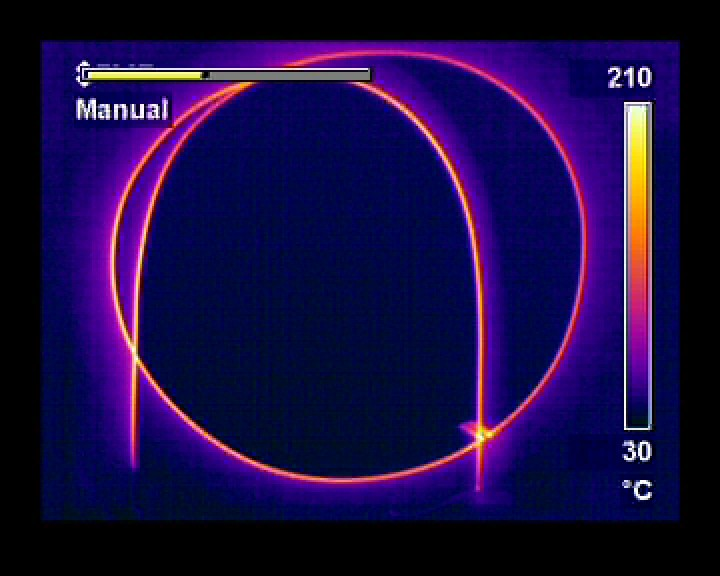
\includegraphics[width=8.5cm]{thermal_image}%
\caption{\label{fig:ThermImg}A thermal image of the coaxial heater.}%
\end{figure}

To quantify the non-uniformity of the coaxial heater, a dual thermocouple probe was inserted into the coaxial heater. The two thermocouples in the probe were 330 mm apart and was in the central third of the coaxial heater. The coaxial heater was submitted to a repeated program of cooling and ballistic heating. Figure \ref{fig:Repeatability} shows that the gradients established by cooling was small (approximately 10 C$^\circ$), stable and repeatable, and should not prevent good chromatography from happening. 

\begin{figure}
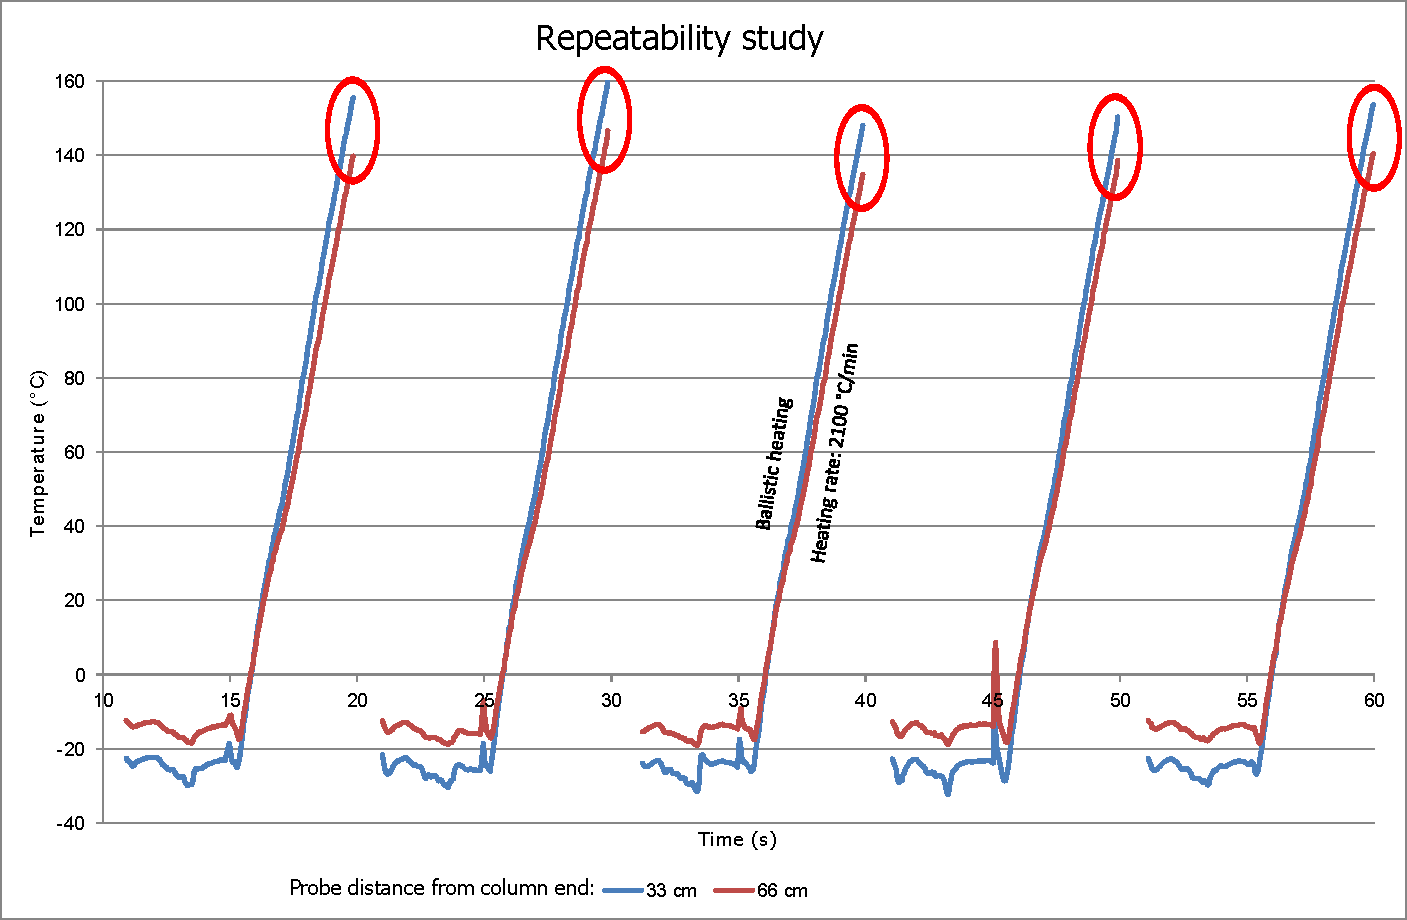
\includegraphics[width=8.5cm]{cp}%
\caption{\label{fig:Repeatability}A graph indicating that temperature gradients are modest, stable and repeatable}%
\end{figure}

\subsection{Temperature calibration}

While it is entirely possible to have a fast temperature program by using the voltage/current ratio alone as a temperature indicator and controlled parameter, it would not be practical to design chromatographic methods or translate methods without a knowledge of the real temperature. Therefore we went to some effort to calibrate the coaxial heater. 

A necessary requirement of calibrating a thermometer is that the thermometer and its calibration environment need to be in equilibrium. The method of our calibration makes this requirement hard to meet, because a single point (the junction of the thermocouple) needs to be in equilibrium with the length of the coaxial heater. This would be very difficult to maintain, especially because the uniformity of heating cannot be guaranteed, and is additionally influenced by the presence of the manifold heaters. For a totally uniform heating of the coaxial heater the manifolds would have to be at the same temperature as the coaxial heater. Under conditions of use the manifolds would be at a higher temperature than the heater, making the calibration invalid. 

However, to make progress, we decided to be pragmatic about the calibration. We did some experiments to determine how much of a temperature difference can be generated in the coaxial heater. A dual-thermocouple probe was constructed, and used to measure temperatures 330 mm apart in the coaxial heater. Using this we could determine that the temperature gradients along the length of the coaxial heater generated by heating and cooling was modest, stable and repeatable. 


This convinced us that a resistance measurement calibrated against temperature would furnish a useful measure of real temperature, although not perfectly accurate. 

The calibration curve is oddly curved, for reasons we don't understand. This being a pragmatic calibration, we fitted a B-spline to the data points, by eye. This procedure can be automated \cite{WenniZheng2012}. Points from this B-spline curve was then extracted to create a calibration curve, from which an estimate of the temperature can be calculated by linear interpolation. 

\begin{figure}
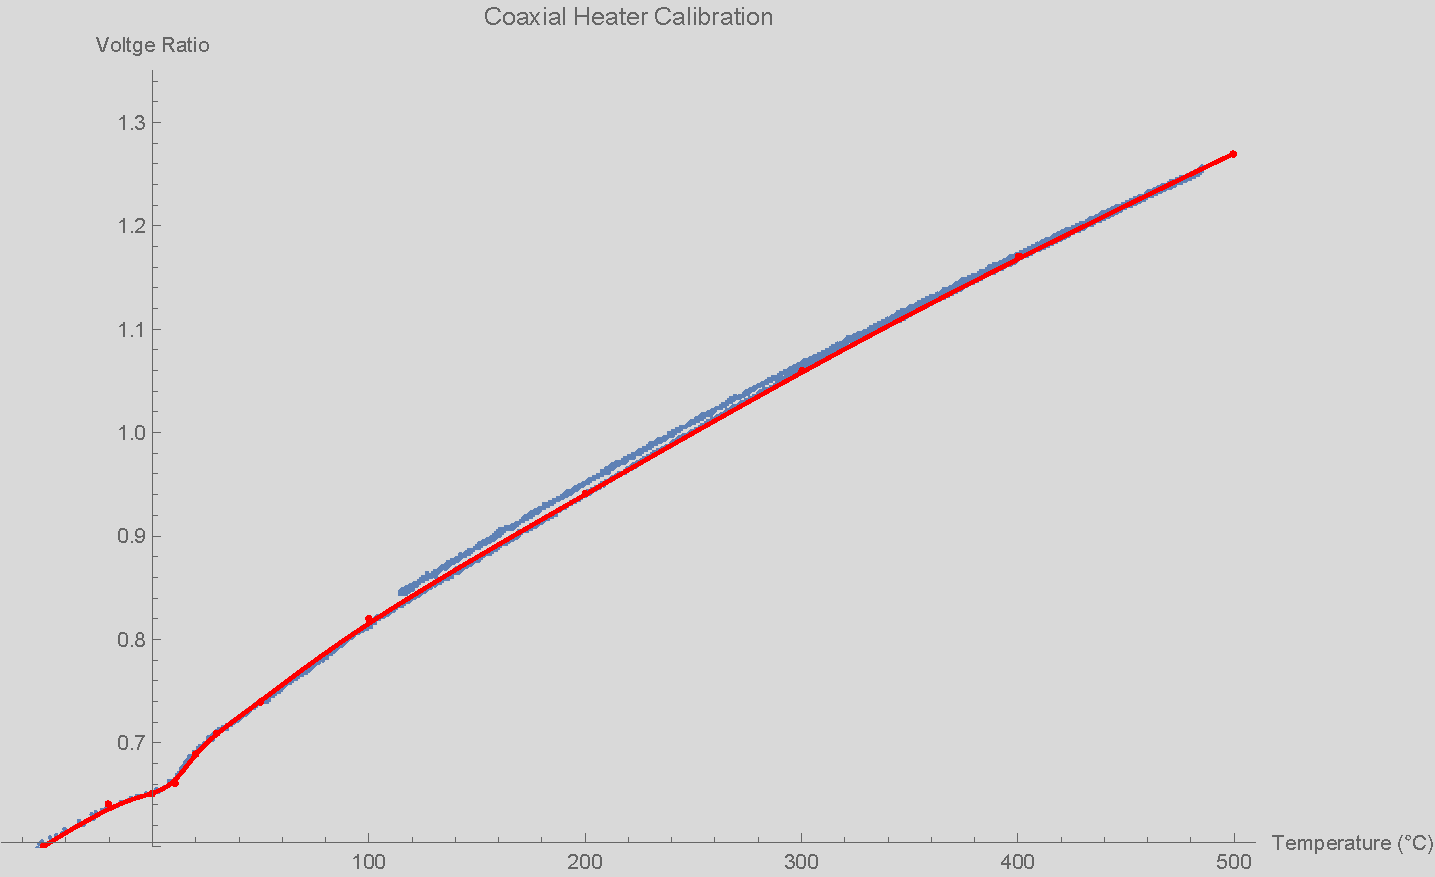
\includegraphics[width=8.5cm]{2015_04_24_Calibration}%
\caption{\label{TempCal}A calibration curve.}%
\end{figure}

\subsection{Heating rate}

According to Blumberg and Klee, a good initial heating rate is 10 C$^\circ$ per void time. Under usual conditions for fast chromatography, according to Venter, this means a heating rate of more than 1000 C$^\circ$/min. Since fast chromatography is a trade-off between excess peak capacity (resolution) for shorter run times, higher heating rates may be required. At a fast linear velocity of 20 cm/s, the void time  of a 1 m column is 5 s, so the 10 C$^\circ$ per 5 s, which is 2 C$^\circ$/s, or 120

The attainable heating rate is a function of power to the heater and of the temperature required. In the instrument presented here power was limited by the range of the DAC of the card. We we able to maintain controlled heating rates of up to 2500 C$^\circ$/min up to 400$^\circ$C, or up to 4000 C$^\circ$/min up to 300 $^\circ$C. (Figure \ref{fig:MaxHeatingRate})

The heating rate attainable then seems to be sufficient for the most demanding fast gas chromatography. 

\begin{figure}
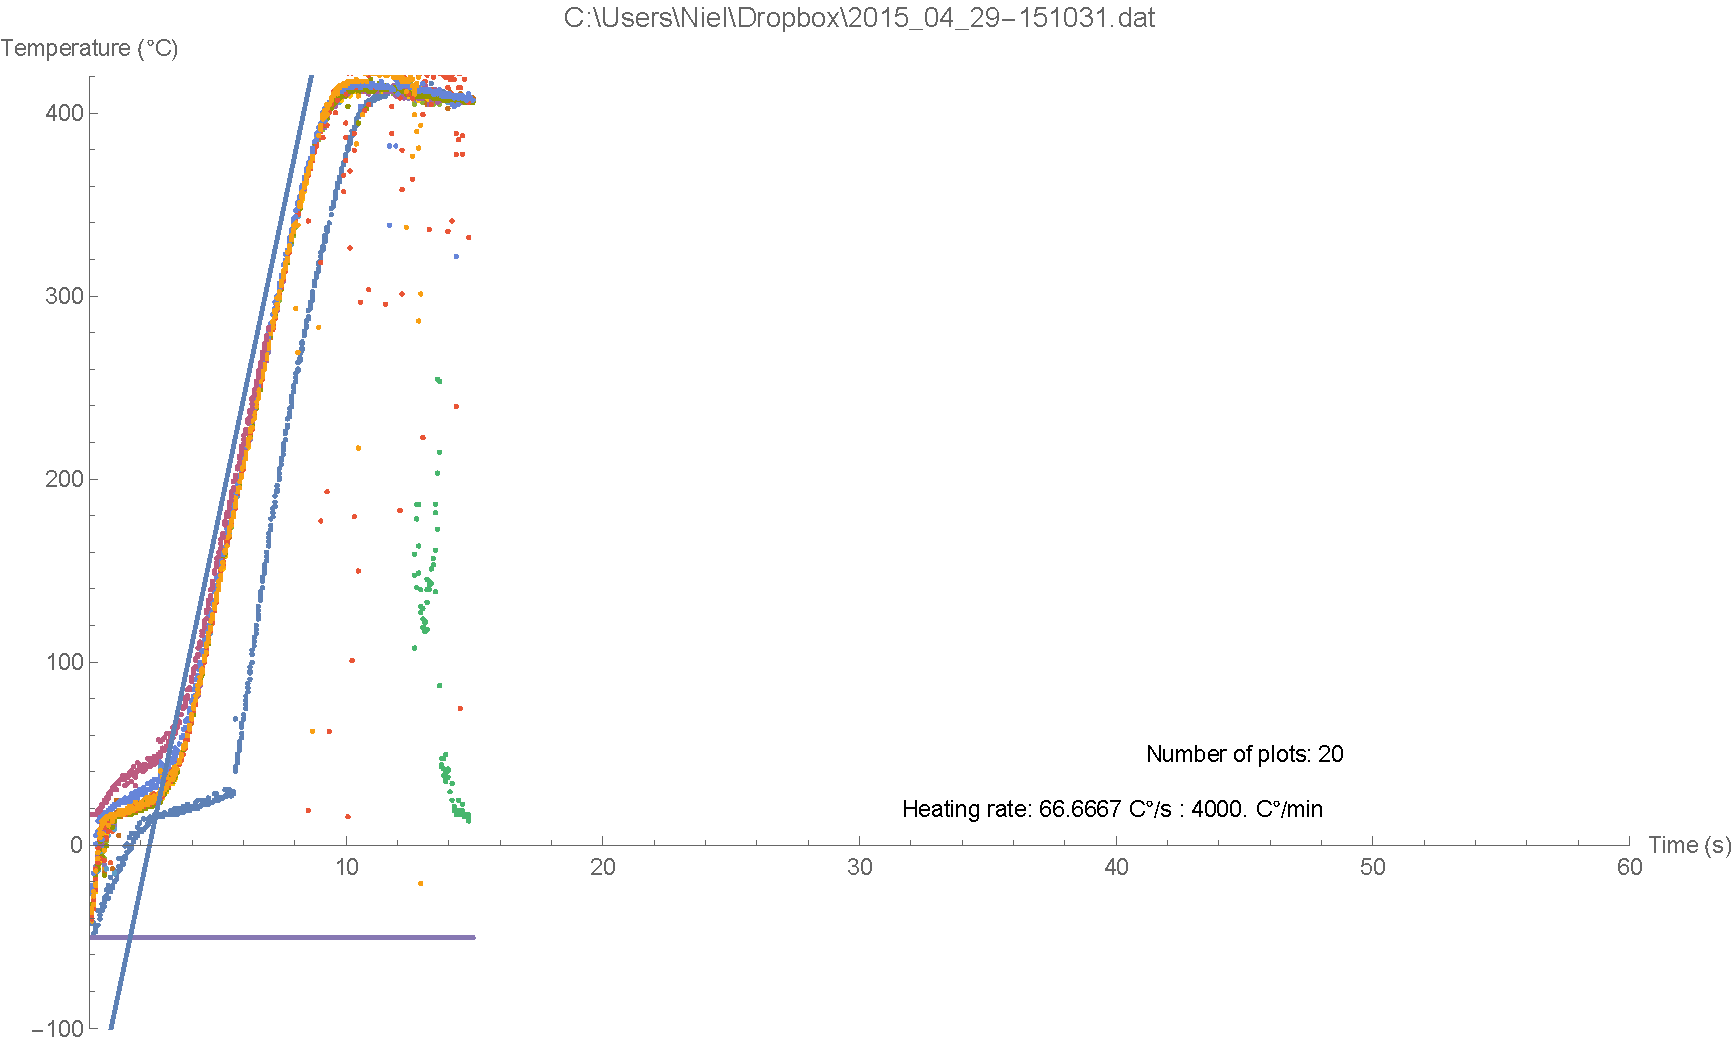
\includegraphics[width=8.5cm]{2015_04_30_Rate_analysis_4000}%
\caption{\label{fig:MaxHeatingRate}Heating rate illustration}%
\end{figure}

\subsection{Cooling rate}

Using evaporating carbon dioxide as a powerful coolant, it was possible to cool down the column at a rate of 5100 C$^\circ$/min. The cooling rate depends on the setting of the metering valve, with the best cooling achieved at an intermediate flow. At high flows the coaxial heater fills with liquid carbon dioxide, with evaporation taking place only at the outlet end. At low flow, evaporation takes place only at the inlet end, the rest of the coaxial heater being filled with gaseous carbon dioxide. This was easily deduced by observing the layer of frost from atmospheric water forming on the coaxial heater. Under ideal conditions the frost would form a continuous layer on the outside of the coaxial heater, which also gave the lowest temperature and best cooling rate.

\subsection{Chromatography}

The chromatographic abilities of the instrument is demonstrated with this cool example. A B50 diesel blend (50:50 biodiesel/diesel) was chromatographed in the described system. The system easily separates the hydrocarbons of the petro-diesel from the fatty acid methyl esters of the biodiesel, and further separate the biodiesel according to the number of double bonds and chain length. 

\begin{figure}
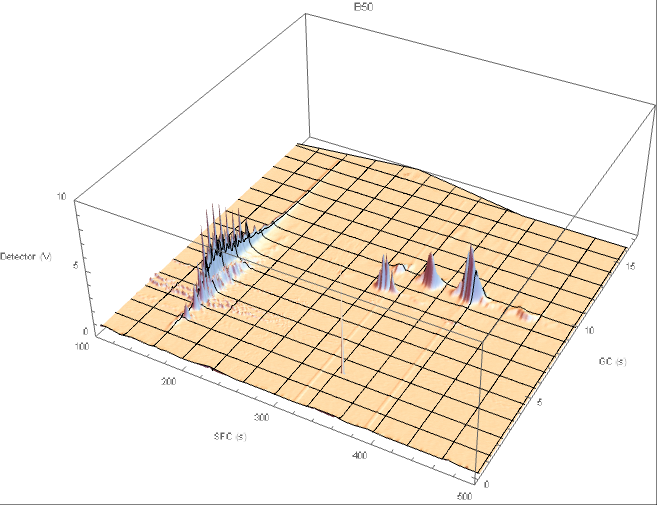
\includegraphics[width=8.5cm]{2DChromatogram_2013_11_29}%
\caption{\label{fig:2DChromatogram}2D chromatogram }%
\end{figure}


\section{Conclusion}

The instrument gives a superb performance, and our cooling is the best coolest cooling in the world. 
\
% If in two-column mode, this environment will change to single-column format so that long equations can be displayed. 
% Use only when necessary.
%\begin{widetext}
%$$\mbox{put long equation here}$$
%\end{widetext}

% Figures should be put into the text as floats. 
% Use the graphics or graphicx packages (distributed with LaTeX2e). EPSFig is no longer fully supported.
% See the LaTeX Graphics Companion by Michel Goosens, Sebastian Rahtz, and Frank Mittelbach for examples. 
%
% Here is an example of the general form of a figure:
% Fill in the caption in the braces of the \caption{} command. 
% Put the label that you will use with \ref{} command in the braces of the \label{} command.
%
% \begin{figure}
% \includegraphics{}% % Important NOTE: Please make certain your figures do not include local directory paths. ex. "c:\file\sub\fig1.eps"
% \caption{\label{}}%
% \end{figure}

% Tables may be be put in the text as floats.
% Here is an example of the general form of a table:
% Fill in the caption in the braces of the \caption{} command. Put the label
% that you will use with \ref{} command in the braces of the \label{} command.
% Insert the column specifiers (l, r, c, d, etc.) in the empty braces of the
% \begin{tabular}{} command.
%
% \begin{table}
% \caption{\label{} }
% \begin{tabular}{}
% \end{tabular}
% \end{table}

% If you have acknowledgments, this puts in the proper section head.

\begin{acknowledgments}
Dr Walter Meyer of the Department of Physics at the University of Pretoria supplied the idea for the electronics that measure the resistance of the stainless steel heating tube. 
%Put your acknowledgments here.
\end{acknowledgments}

% Create the reference section using BibTeX:
\bibliography{RSI-2014_01Bib}
% Run this once to generate your BBL file. Then copy the contents of your BBL file into your main latex file, commenting out "\bibliography"

\end{document}
%
% ****** End of file aiptemplate.tex ******
